\documentclass[12pt,a4paper]{article}
%packages
\usepackage[utf8]{inputenc}
\usepackage[T1]{fontenc}
\usepackage[english]{babel}
\usepackage{amsmath}
\usepackage{amsfonts}
\usepackage{amssymb}
\usepackage{graphicx}
\usepackage{hyperref}
\usepackage{tikz}
\usetikzlibrary{positioning,angles,quotes}
\usepackage[acronym]{glossaries}
%glossary 
\newacronym{qrl}{QRL}{Quantum Reinforcement Learning}
\newacronym{ai}{AI}{Artificial Intelligence}
\newacronym{drl}{DRL}{Deep Reinforcement Learning}
\newacronym{rl}{RL}{Reinforcement Learning}
\newacronym{qc}{QC}{Quantum Computing}
\newacronym{nn}{NN}{Neural Networks}
\newacronym{mdp}{MDP}{Markov Decision Process}
\newacronym{vqa}{VQA}{Variational Quantum Algorithm}
\makenoidxglossaries
%settings
\usepackage[left=2.00cm, right=2.00cm, top=2.00cm, bottom=2.00cm]{geometry}
\author{Matteo Conterno}
\title{Prospects of quantum computing approach to reinforcement learning}
%start of document
\begin{document}
	\maketitle
	\begin{center}
	\section*{Abstract}
\end{center}
Reinforcement learning is one of three major techniques that allows a model to learn, especially this technique focus on how to create an optimal agent able to reach an objective by interacting with an environment. 
This thesis tries to analyze the possible potentials and advantages that would derive by using quantum circuits with neural networks; 
analyzing and explaining how it is possible to create hybrid algorithms that exploit the advantages of both the classical and quantum algorithm, expanding the applicability not only on simulators, but even on quantum devices such as Rigetti and IonQ's processors through the amazon AWS braket service. 
Lastly it is analyzed how the quantum noise influence an optimal model obtained through a simulator, by testing it on a quantum processor to understand if it is possible to use the hybrid algorithm on the actual devices.
\newline
\begin{center}
	\printglossary
\end{center}

	{
	 	\hypersetup{hidelinks}
		\tableofcontents
	}
	
	\section{Introduction to Deep Reinforcement Learning and Quantum Computing}
%introduction
This section of the thesis is created so that it can give an introduction to the fields of \acrlong{ai}(\acrshort{ai}) specifically to \acrlong{drl}(\acrshort{drl}) and the basis of \acrlong{qc}(\acrshort{qc}) in order to understand afterward the fusion of these two different fields on \acrlong{qrl}(\acrshort{qrl}). If already expert on these subjects fell free to skip at the next section.
%subsection of learnings
\subsection{Approaches of learning}
Currently to make an algorithm learn the following components are required:
\begin{itemize}
	\item Data
	\item Model
	\item Approach of learning
\end{itemize}
The data is necessary in every model that uses some learning approach, the amount and quality can heavily influence on the model ability to correctly and efficiently reach his goal. 
The model is an algorithm that, given some data and a predefined objective, tries to complete his task using some approach of learning. In order to check that the model has correctly learned it will be later tested on unseen data and evaluated to understand if it is able to replicate the performances given a similar dataset.\\
The approach of learning specify how the model can learn to complete his task. At the moment there are three major ways:
\begin{itemize}
	\item \textbf{Supervised learning} : the dataset given is already labeled, this means that we can define when the model is incorrect or correct.
	\item \textbf{Unspervised learning} : the dataset is not labeled, this means that we can't define easily when the model is correct or incorrect and the model must uncover some pattern.
	\item \textbf{Reinforcement learning} : an agent interact with the environment in order to become the most optimal agent to complete the task.
\end{itemize}
This thesis will focalize mainly on the reinforcement learning approach and especially on the \acrfull{drl} which uses \acrfull{nn} to define the most optimal agent.
In this thesis the focus is on what kind of advantage we can obtain by using a quantum algorithm such as \acrfull{vqa}, this can be used in other context and application. Futhermore it has been demostrated that \acrshort{vqa} and \acrshort{nn} share some similarities and properties. The main drawback is the fact that when a \acrshort{vqa} is trained on a classical device, there is a major overhead of time due to simulation of the quantum circuit implemented and the number of qubits is limited.
\newpage
%sub section of reinforcement learning
\subsection{Reinforcement Learning}
As said earlier a reinforcement learning approach consist of creating the most optimal agent able to complete a predefined task by interacting with the environment and taking some action. Questions arises about: how do we define correctly what is the correct action? How do we model a dynamic environment? Futhermore how do we define when an action is good or bad? The answer is given by using a staristical model called \acrfull{mdp} .
\subsubsection{Markov Decision Process}
In order to model a dynamic environment with a model whose action can influence the sistem it is necessary to use the \acrfull{mdp} which is an extension of Markov chains; these are a stochastic model that is able to describe a sequence of possible events that satisfy the Markov propriety, that is each event depends only on the previous event.\\
It is necessary to note that an \acrshort{mdp} is based on Markov Chains that not only model the states, but even the time and this can be defined as continuous or discretized, for this thesis we will focalize on the discrete case.
\acrshort{mdp} is an extension of Markov Chains because we have an agent which can influence the state of environment and outcome, so we need to have a framework to define his decision making. An \acrshort{mdp} is defined as a 4-tuple containing the following elements:
\begin{itemize}
	\item $S$ : set of states
	\item $A$ : set of actions
	\item $P_a (s, s') = Pr(s_{t+1} = s' \vert s_{t} = s)$ : is the transition probability of going from state $s$ to $s'$ by taking an action $a$
	\item $R_{a}(s,s')$ is the immediate reward obtained by transitioning from state $s$ to $s'$ by action $a$
\end{itemize}
The difference with a Markov chains is the missing elements $P_a (s, s')$ and $R_{a}(s,s')$ which are necessary for the decision process, to see an example graph of and MDP see Figure \ref{fig:mdpgraph}.
\begin{figure}[h!]
	\centering
	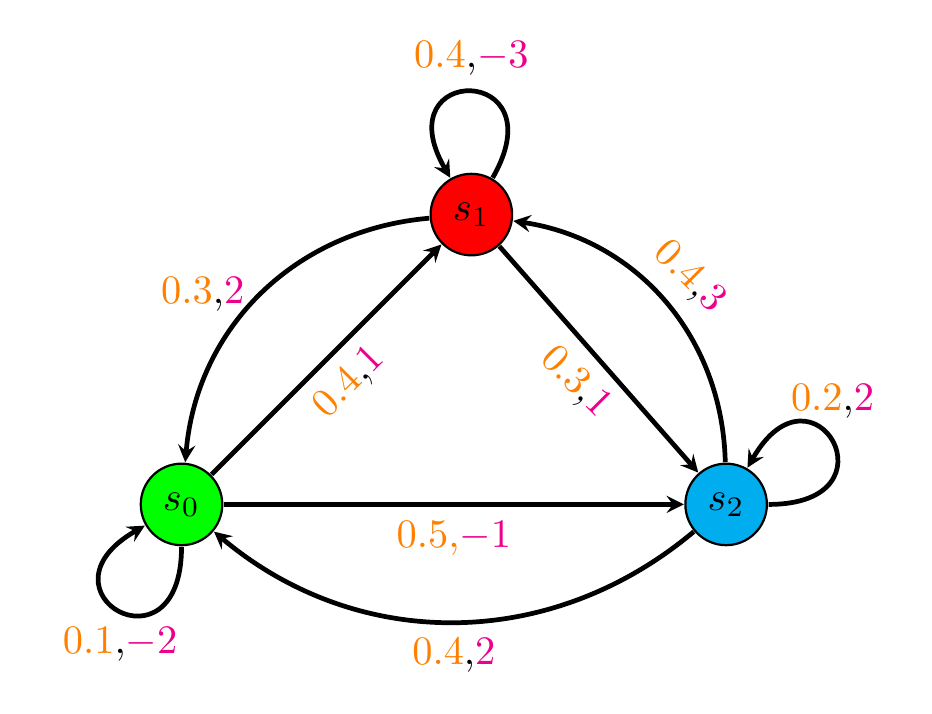
\begin{tikzpicture}[thick,scale=1.46, every node/.style={transform shape}, line width=0.6mm]
		\tikzstyle{round}=[thick,draw=black,circle]
		\node[round, fill=green] (s0) {$s_0$};
		\node[round,above right=20mm and 20mm of s0, fill=red] (s1) {$s_1$};
		\node[round, right=40mm of s0, fill=cyan] (s2) {$s_2$};
		\draw[-stealth] (s0) -- node[below, rotate=45]
		{\color{orange} $0.4$\color{black},\color{magenta} $1$} (s1);
		\draw[-stealth] (s0) -- node[below]
		{\color{orange} $0.5$,\color{magenta} $-1$} (s2);
		\draw[-stealth] (s1) [bend right=40] to node[left]
		{\color{orange} $0.3$\color{black},\color{magenta} $2$}(s0) ;
		\draw[-stealth] (s1) -- node[below, rotate=-45]
		{\color{orange} $0.3$\color{black},\color{magenta} $1$} (s2) ;
		\draw[-stealth] (s2) [bend left=40]  to node[below]
		{\color{orange} $0.4$\color{black},\color{magenta} $2$} (s0);
		\draw[-stealth] (s2) [bend right=40] to node[above, rotate=-45]
		{\color{orange} $0.4$\color{black},\color{magenta} $3$} (s1);
		\draw[-stealth] (s0) [out=-90,in=-150,loop] to node[below]
		{\color{orange} $0.1$\color{black},\color{magenta} $-2$} (s0) ;
		\draw[-stealth] (s1) [out=60,in=120,loop] to node[above]
		{\color{orange} $0.4$\color{black},\color{magenta} $-3$}(s1);
		\draw[-stealth] (s2) [out=0,in=60,loop] to node[above=2pt]
		{\color{orange} $0.2$\color{black},\color{magenta} $2$}(s2);
	\end{tikzpicture}
	\caption[MDP Graph]{Markov decision process graph, transition probability is in orange and reward in magenta.}
	\label{fig:mdpgraph}
\end{figure}
\\
The interaction between agent and environment can be defined by time, using a discrete step which implies view it as distinct separate points in time uniquely definied and to which a single state value can be associated.
The sequence of observation over times form a chain of states that is called \textbf{history}, this will be particularly important because it will be used later to define the transition probability and use it later to model the interaction with environment.\\
In order to include the reward element of an \acrshort{mdp} accumulated from present and future a new quantity need to be defined called \textbf{return}:
\begin{equation}\label{return}
	G_t = R_{t+1} + \gamma R_{t+2} + \dots = \sum_{k=0}^{\infty} \gamma^{k} R_{t+k}
\end{equation}
The $\gamma$ is a variable called discount factore with values limited inside the range of 0 and 1 with extremes included, i.e. $\gamma \in [0,1]$. The scope of this variable is to limit the horizon of \textbf{return}, in case $\gamma$ is equal to 0 only the immediate reward will be counted and when it is 1 infinite future steps will be considered.Usually the literature use $\gamma \in [0.9, 0.999]$ in order to gradually consider less relevant further time steps rewards thanks to the k-power of $\gamma$ inside \ref{return}.
The RL learning approach has the objective to maximize the \textbf{return} quantity, but this form is not useful for the agent due to the fact that it considers every possible chain that can be observed using the Markov reward process. This means that it can vary widely even for the same state, however it is possible to calculate the expectation of return from any state by averaging a large number of chains and obtain a new quantity called \textbf{value of state}:
\begin{equation}
	V(s) = \mathbb{E}[G | S_t = s] = \mathbb{E}[\sum_{t=0}^{\infty} r_t \gamma^t]
\end{equation}
These formulas considers the reward and state but they are not sufficient to model envrinoment and agent, so it is necessary to define a set of rules to control the agent behaviour with the objective of RL that is to maximize the return, for these reasons a new quantity must be defined \textbf{policy}.It is formally determined as probability distribution over actions for every possible state, i.e.:
\begin{equation}\label{policy}
	\pi(a|s) = P[A_t = a | S_t = s]
\end{equation}
The policy is defined as a probability to introduce randomness of the agent that will be useful during the training phase, furthermore if policy is fixed the transition and reward matrixes can be reduced using policy's probabilities reducing the action dimension.
\subsubsection{Value iteration}
As stated before the objective of RL is to maximize the return, problem is how to approximate the best optimal policy and values state in order to define the correct actions for given state. Fortunately the \textbf{Bellman optimality equation} is able to estimate approximately the best action to take on deterministic and statistical case.The equation for a general case is defined as:
\begin{equation}\label{bellman}
	V(s) = \max_{a \in A} \mathbb{E}_{s' \sim S}[(s,a) + \gamma V(s')] = \max_{a \in A} \sum_{s' \in S} p_{a, s \to s'}(r(s,a) + \gamma V(s'))
\end{equation}
The interpretation of this formula is that the optimal value state is equal to the action which gives the maximum possible expected immediate reward, plus the discounted long-term reward of next state. Futhermore this definition is recursive because the value state is determined from values of immediate reachable states. This formula not only gives the best reward that can be obtained, but it gives the best policy to obtain that reward.
In order to simplify this formula it is possible to define other quantities, such as \textbf{value of action}:
\begin{equation}\label{action value}
	Q(s,a) = \mathbb{E}_{s' \sim S}[r(s,a)+ \gamma V(s')] = \sum_{s' \in S} p_{a, s \to s'}(r(s,a) + \gamma V(s'))
\end{equation}
This quantity allow to define a pair of state and action, it is particulary important because it defines a category of learning called \textbf{Q-learning} which will be the focus of this thesis. As you can see using this new definition \ref{bellman} becomes:
\begin{equation*}
	V(s) = \max_{a \in A} Q(s,a)
\end{equation*}
Thanks to this, the \ref{action value} can be even defined recursively and this will be particulary useful later to use it along the deep learning approach:
\begin{equation}\label{recursive}
	Q(s,a) = r(s,a) + \gamma \max_{a \in A} Q(s',a')
\end{equation} 

\end{document}